\documentclass[twoside, 11pt]{article}
\usepackage{titlesec}

%\setcounter{secnumdepth}{0}
%\titleformat{\section}[block]{\Large\bfseries\filcenter}{}{1em}{}
%\titleformat{\subsection}[hang]{\large\bfseries}{}{1em}{}
%%\usepackage{../estilo-apuntes}
%\AtBeginDocument{%
%  \renewcommand\tablename{Tabla}
%}
%\newcommand{\yields}{\overset{\Pi,I^*}{\rightarrow}}
%\newcommand{\yieldsone}{\overset{\Pi,I}{\rightarrow}}
%\newcommand{\yieldsn}{\overset{\Pi,I^n}{\rightarrow}}
%


%------------------------------------------------------------------------
\usepackage[utf8x]{inputenc}
\usepackage[spanish,es-nodecimaldot]{babel}
\usepackage{amsmath,amssymb,amsthm,amsfonts}
\usepackage{enumerate}
\usepackage{mathrsfs}
\usepackage{bm}
\usepackage{array,multirow}
\usepackage{fancyhdr}
\usepackage{titlesec}
\usepackage{floatrow}
\usepackage{makeidx}
\usepackage[tocflat]{tocstyle}
\usetocstyle{standard}
\usepackage{subfiles}
\usepackage{color}
\usepackage{hyperref}
\hypersetup{colorlinks=true,citecolor=red, linkcolor=blue}
\usepackage[]{graphicx}
\usepackage{pgf,tikz}
\usepackage{tikz-cd}
\usetikzlibrary{babel}
\usetikzlibrary{arrows}
\usetikzlibrary{cd}

\renewcommand{\baselinestretch}{1,1}
\setlength{\oddsidemargin}{0.25in}
\setlength{\evensidemargin}{0.25in}
\setlength{\textwidth}{6in}
\setlength{\topmargin}{0.1in}
\setlength{\headheight}{0.1in}
\setlength{\headsep}{0.1in}
\setlength{\textheight}{8in}
\setlength{\footskip}{0.75in}

\theoremstyle{definition}

\newtheorem{teorema}{Teorema}[section]
\newtheorem{defi}[teorema]{Definición}
\newtheorem{coro}[teorema]{Corolario}
\newtheorem{lemma}[teorema]{Lema}
\newtheorem{ej}[teorema]{Ejemplo}
\newtheorem{ejs}[teorema]{Ejemplos}
\newtheorem{observacion}[teorema]{Observación}
\newtheorem{observaciones}[teorema]{Observaciones}
\newtheorem{prop}[teorema]{Proposición}
\newtheorem{propi}[teorema]{Propiedades}
\newtheorem{nota}[teorema]{Nota}
\newtheorem{notas}[teorema]{Notas}
\newtheorem*{dem}{Demostración}
\newtheorem{ejer}[teorema]{Ejercicio}
\newtheorem{consec}[teorema]{Consecuencia}
\newtheorem{consecs}[teorema]{Consecuencias}
\newtheorem{reco}[teorema]{Recordatorio}

\SetUnicodeOption{mathletters}
\SetUnicodeOption{autogenerated}
\PrerenderUnicode{áéíóú}
\DeclareMathOperator{\cardinal}{card}

\providecommand{\card}[1]{\cardinal\left(#1\right)}

\providecommand{\abs}[1]{\left|#1\right|}
\providecommand{\sen}[1]{sen #1}
\providecommand{\norm}[1]{\left\lVert#1\right\rVert}
\providecommand{\ninf}[1]{\norm{#1}_\infty}
\providecommand{\numn}[1]{\norm{#1}_1}
\providecommand{\gabs}[1]{\left|{#1}\right|}
\newcommand{\bor}[1]{\mathcal{B}(#1)}
\newcommand{\A}{\mathbb{A}}
\newcommand{\calA}{\mathcal{A}}
\newcommand{\calF}{\mathcal{F}}
\newcommand{\calG}{\mathcal{G}}
\newcommand{\Ank}{\A^n_k}
\newcommand{\Amk}{\A^m_k}
\newcommand{\R}{\mathbb{R}}
\newcommand{\Z}{\mathbb{Z}}
\newcommand{\F}{\mathbb{F}}
\newcommand{\N}{\mathbb{N}}
\newcommand{\PP}{\mathbb{P}}
\newcommand{\Pnk}{\PP^n_k}
\newcommand{\Pmk}{\PP^m_k}
\newcommand{\Q}{\mathbb{Q}}
\newcommand{\C}{\mathbb{C}}
\newcommand{\CC}{\mathcal{C}}
\newcommand{\K}{\mathbb{K}}
\newcommand{\KK}{{\mathcal K}}
\newcommand{\OO}{{\mathcal O}}
\newcommand{\X}{\mathbb{X}}
\newcommand{\Y}{\mathbb{Y}}
\newcommand{\Va}{\mathcal{V}_{a}}
\newcommand{\Vp}{\mathcal{V}_{p}}
\newcommand{\V}{\mathcal{V}}
\newcommand{\I}{\mathcal{I}}
\newcommand{\m}{{\mathfrak{m}}}
\newcommand{\p}{{\mathfrak{p}}}
\newcommand{\Tau}{\mathcal{T}}
\newcommand{\parcial}[2]{\frac{\partial #1}{\partial #2}}
\newcommand{\dparcial}[2]{\dfrac{\partial #1}{\partial #2}}
\DeclareMathOperator{\Ima}{Im}
\DeclareMathOperator{\Rea}{Re}
\DeclareMathOperator{\coker}{coker}

%--------------------------------------------------------------







\rhead{Geometría Semi-Riemanniana (Máster Universitario en Matemáticas)}
\lhead{Curso 2018/2019}

\begin{document}
\begin{titlepage}
	\centering
	{\huge\bfseries Geometría Semi-Riemanniana \par}
	\vspace{1cm}
	{\Huge\bfseries El cilindro \par}
	\vspace{1cm}
	{\Large Javier Aguilar Martín\par}
	\vspace{1cm}
	{\large \today\par}
	\vspace{1cm}

\begin{abstract}
\normalsize
Este trabajo consiste en desarrollar un ejemplo en el que se repasan los principales conceptos sobre Variedades Diferenciables y Geometría Riemanniana, concretamente el cilindro. 
\end{abstract}

	\vfill
	{\small Esta obra está licenciada bajo la Licencia Creative Commons Atribución 3.0 España. Para ver una copia de esta licencia, visite \url{http://creativecommons.org/licenses/by/3.0/es/} o envíe una carta a Creative Commons, PO Box 1866, Mountain View, CA 94042, USA.

\bigskip

Usted es libre de:
\begin{itemize}
 \item copiar, distribuir y comunicar públicamente la obra
\item hacer obras derivadas
\end{itemize}

Bajo las condiciones siguientes:
\begin{itemize}
 \item {\bf Reconocimiento:} Debe reconocer los créditos de la obra maestra especificada por el autor o el licenciador (pero no de una manera que sugiera que tiene su apoyo o apoyan el uso que hace de su obra).
 \item {\bf No comercial:} No puede utilizar esta obra para fines comerciales.
\item {\bf Compartir bajo la misma licencia:} Si altera o transforma esta obra, o genera una obra derivada, sólo puede distribuir la obra generada bajo una licencia idéntica a ésta.
\end{itemize}}

	
\end{titlepage}

\tableofcontents

\newpage

\section{Dos estructuras de variedad diferenciable compatibles}

Definimos el cilindro de radio $r$ como el subespacio euclídeo $C=\{(x,y,z)\in\R^3\mid x^2+y^2=r^2\}$. En este trabajo nos vamos a quedar en el caso $r=1$ por sencillez, pero todos los resultados son análogos para cualquier $r>0$. Vamos a ver que podemos dotar al cilindro de al menos dos estructuras diferenciables compatibles. Será útil recordar que hay una parametrización del cilindro $p:(0,2\pi)\times\R\to C$ dada por $p(\theta,t)=(\cos\theta,\sin\theta, t)$ y que podemos cubrir el cilindro por completo añadiendo otra parametrización igual cambiando el intervalo $(0,2\pi)$ por $(-\pi,\pi)$. 

\subsection{Primera estructura}
%Como sabemos por los cursos del Grado y además es fácil comprobar, el cilindro $C$ está parametrizado por $\varphi^{-1}:(-\pi,\pi)\times\R\to C$, donde $\varphi^{-1}(\theta,t)=(\cos\theta,\sin\theta, t)$. Para cubrir todo el cilindro necesitamos otra parametrización más, $\psi^{-1}:(0,2\pi)\times\R\to C$ definida de la misma forma que $\varphi^{-1}$. Por tanto, para dotar al cilindro de estructura de variedad diferenciable basta tomar las inversas de estas parametrizaciones. Denotamos $r_\varphi$ y $r_\psi$ respectivamente a las rectas verticales que dejan sin cubrir las parametrizaciones $\varphi^{-1}$ y $\psi^{-1}$. Sea entonces $\varphi:C\setminus r_\varphi\to(-\pi,\pi)\times\R$ dada por $\varphi(x,y,z)=(\arccos x-\pi, z)$ y $\psi:C\setminus r_\psi\to(0,2\pi)\times\R$ dada por $\psi(x,y,z)=(\arccos x, z)$. Las cartas están claramente relacionadas, ya que el cambio de cartas es simplemente el desfase de ángulo entre una y otra. 

Vamos a darle primero la estructura de variedad diferenciable como variedad producto $S^1\times\R$, por lo que bastará tomar las cartas de $S^1$ y añadirle la identidad en la última coordenada. Tenemos entonces cuatro cartas $\varphi_i$, $i=1,2,3,4$ definidas mediante
\[
\varphi_1:C_1\times\R\to(0,\pi)\times\R; \varphi(x,y,z)=(\arccos(x),z)
\]
\[
\varphi_2:C_2\times\R\to\left(-\frac{\pi}{2},\frac{\pi}{2}\right)\times\R; \varphi(x,y,z)=(\arcsin(y),z)
\]
\[
\varphi_3:C_3\times\R\to(-\pi,0)\times\R; \varphi(x,y,z)=(\arccos(x)-\pi,z)
\]
\[
\varphi_2:C_4\times\R\to\left(\frac{\pi}{2},\frac{3\pi}{2}\right)\times\R; \varphi(x,y,z)=(\arcsin(y)+\pi,z)
\]

donde $C_1$ es la semicircunferencia abierta superior, $C_2$ la derecha, $C_3$ la inferior y $C_4$ la izquierda. Es sencillo probar que las cartas efectivamente están relacionadas.

\begin{figure}[h!]
\definecolor{ffdxqq}{rgb}{1.,0.8431372549019608,0.}
\definecolor{qqqqff}{rgb}{0.,0.,1.}
\definecolor{ffqqqq}{rgb}{1.,0.,0.}
\definecolor{qqffqq}{rgb}{0.,1.,0.}
\begin{tikzpicture}[line cap=round,line join=round,>=triangle 45,x=1.0cm,y=1.0cm]
\clip(-2.5,-2.7925) rectangle (2.8175,2.545);
\draw [line width=2.pt] (0.,0.) circle (2.cm);
\draw [shift={(0.005,0.015)},line width=4.4pt,color=qqffqq]  plot[domain=-0.006896442388348412:3.1346962112014447,variable=\t]({1.*2.1750517235229143*cos(\t r)+0.*2.1750517235229143*sin(\t r)},{0.*2.1750517235229143*cos(\t r)+1.*2.1750517235229143*sin(\t r)});
\draw [shift={(0.005,0.015)},line width=4.pt,color=ffqqqq]  plot[domain=3.1346962112014447:6.276288864791238,variable=\t]({1.*2.1750517235229143*cos(\t r)+0.*2.1750517235229143*sin(\t r)},{0.*2.1750517235229143*cos(\t r)+1.*2.1750517235229143*sin(\t r)});
\draw [shift={(0.,0.03)},line width=4.4pt,color=qqqqff]  plot[domain=-1.5707963267948966:1.5707963267948966,variable=\t]({1.*2.34*cos(\t r)+0.*2.34*sin(\t r)},{0.*2.34*cos(\t r)+1.*2.34*sin(\t r)});
\draw [shift={(0.,0.03)},line width=4.4pt,color=ffdxqq]  plot[domain=1.5707963267948966:4.71238898038469,variable=\t]({1.*2.34*cos(\t r)+0.*2.34*sin(\t r)},{0.*2.34*cos(\t r)+1.*2.34*sin(\t r)});
\end{tikzpicture}
\caption{En {\color{green}verde} el dominio de {\color{green}$\varphi_1$}, en {\color{blue}azul} el de {\color{blue}$\varphi_2$}, en {\color{red}rojo} el de  {\color{red}$\varphi_3$} y en {\color{yellow}amarillo} el de {\color{yellow}$\varphi_4$}.}
\end{figure}
%HACER DIBUJO

\subsection{Segunda estructura}


%Obsérvese que la estructura de variedad diferenciable anterior que le hemos dado al cilindro coincide salvo elección de dominio con las estructuras que tiene como variedad producto $S^1\times \R$, como superficie de revolución generada por la recta $\alpha(t)=(1,0,t)$ y como superficie reglada generada por la curva $\alpha(\theta)=(\cos\theta,\sin\theta, 0)$ y el vector $(0,0,1)$. Así que podríamos dar cualquiera de estas estructuras y sería trivialmente compatible con la anterior. De modo que vamos a dar otra diferente que no sea tan trivial.

Consideremos la aplicación $\psi^{-1}:\R^2 \setminus\{0\}\to C$ dada por $$\psi^{-1}(x,y)=\left(\frac{x}{\sqrt{x^2+y^2}},\frac{y}{\sqrt{x^2+y^2}}, \log\sqrt{x^2+y^2} \right),$$ consistente en transformar las semirrectas que parten del origen de $\R^2$ en las líneas verticales del cilindro. Esta aplicación es claramente diferenciable como aplicación $\R^2\to\R^3$, y vamos a ver que tiene una inversa diferenciable, que será la carta que formará el nuevo atlas diferenciable. Basta tomar $\psi:C\to\R^2\setminus\{0\}$ definida como $$\psi(x,y,z)=(xe^z,ye^z).$$ 

\subsection{Compatibilidad}

Comprobamos que las cartas $(C, \psi)$ y $(C_i\times\R, \varphi_i)$ están relacionadas. Basta hacerlo para $i=1$, pues el resto son análogos. Los cambios de cartas

\[
\varphi_1\circ \psi^{-1}: \psi(C_1\times\R)\to \varphi_1(C_1\times\R)
\]
y 
\[
\psi\circ\varphi_1^{-1} : \varphi_1(C_1\times\R)\to \psi(C_1\times\R)
\]
tienen coordenadas definidas como composición de funciones diferenciables en los dominios correspondientes como vamos a ver. Por lo que son diferenciables. 
%Notar que x/raiz <= 1
\[
\varphi_1\circ \psi^{-1}(x,y)=\varphi_1\left(\frac{x}{\sqrt{x^2+y^2}},\frac{y}{\sqrt{x^2+y^2}}, \log\sqrt{x^2+y^2} \right)=\left(\arccos\left(\frac{x}{\sqrt{x^2+y^2}}\right),  \log\sqrt{x^2+y^2} \right)
\]
\[
\psi\circ\varphi_1^{-1}(x,y)=\psi(\cos(x),\sin(x),z)=(\cos(x)e^z,\sin(x)e^z)
\]

\section{Ejemplos de aplicaciones y funciones diferenciables}

\subsection{Aplicaciones diferenciables}
Damos dos ejemplos de aplicaciones diferenciables del cilindro en sí mismo y otra que vaya de otra variedad en el cilindro. Para una vamos a utilizar las coordenadas implícitas del cilindro y para otra la parametrización vista en la primera sección. 


\begin{enumerate}


\item La primera es la que ``le da la vuelta'' al cilindro, es decir, $f:C\to C$ descrita como $f(x,y,z)=(x,y,-z)$. Esta aplicación se puede describir como $Id_{S^1}\times -Id_{\R}:S^1\times\R\to S^1\times\R$. Como cada componente es claramente diferenciable, $f$ es diferenciable. 

\item El segundo ejemplo será una rotación de ángulo $\alpha$, la cual viene dada por la aplicación $g:C\to C$, $g(\cos\theta,\sin\theta, t)=(\cos(\theta+\alpha), \sin(\theta+\alpha), t)$. Se comprueba que al hacer la composición $\psi\circ g\circ \psi^{-1}$ el resultado es diferenciable por ser las componentes producto y composición de funciones diferenciables. 

\item Para esta última aplicación sea $K$ el cono (sin vértice) cuya ecuación implícita es $$x^2+y^2=z^2$$ para $z\neq 0$. Damos la aplicación $h:K\to C$ definida por $x\mapsto \frac{x}{z}, y\mapsto \frac{y}{z}, z\mapsto z$. Es claro que la aplicación está bien dedinida y la imagen está contenida en el cilindro. Ahora, para que tenga sentido hablar de diferenciabilidad, convertimos el cono en una variedad diferenciable mediante las parametrizaciones $\widetilde{\psi}_1^{-1}:(0,2\pi)\times\R^*\to K$ y $\widetilde{\psi}_2^{-1}:(-\pi,\pi)\times\R^*\to K$ definidas ambas por la correspondencia $(s,t)\mapsto (t\cos s, t\sin s, t)$. Vemos que, en el dominio correspondiente, la composición $\psi\circ h\circ \widetilde{\psi}_i^{-1}$ tiene para $i=1,2$  la expresión $(\cos(s)e^t, \sin(s)e^t, e^t)$, que es claramente diferenciable. 

Esta aplicación es la proyección del cono sobre el cilindro. 

%K de Konus en alemán %\R^* son las unidades de \R, o sea todos menos el 0

\end{enumerate}

\subsection{Funciones diferenciables}

Damos ahora también dos ejemplos de funciones diferenciables. 

\begin{enumerate}


\item
 La primera será la proyección sobre la tercera coordenada, es decir, $f:C\to\R$ definida como $f(x,y,z)=z$, que es trivialmente diferenciable. 

\item
 El siguiente ejemplo será $g:C\to\R$ dada por $g(x,y,z)=x+y+z$. Es trivial probar que es diferenciable usando la primera estructura diferenciable. 

\end{enumerate}


\section{Ejemplos de curvas diferenciables y vectores tangentes}



Vamos a dar dos ejemplos de curvas que luego veremos que son geodésicas y uno que se verá que no es geodésica, y calcularemos vectores tangentes a la variedad en puntos por los que pasan estas curvas. Usaremos el sistema de coordenadas de una sola carta $(C, \psi=(x_1,x_2))$ para calcular las coordenadas de los vectores tangentes mediante su expresión local.

%\begin{enumerate}
%
%\item
% La curva $\gamma(t)=(\cos t, \sin t, t)$ con $t\in\R$ es una curva diferenciable sobre el cilindro. Esta curva tiene el vector tangente en cada punto $(-\sin t,\cos t, 1)$. Por ejemplo, para $t=0$, es decir, en el punto $(1,0,0)$, obtenemos el vector $(0,1,1)$. 
%
%\item
% La curva $\beta(t)=(1, 0, t)$ para $t\in\R$ es una curva diferenciable sobre el cilindro. Esta curva tiene como vector tangente el vector $(1,0,1)$ en todo punto.
%
%\item La curva $\sigma(t)=(\cos t, \sin t, t^2)$, $t\in\R$, es una curva diferenciable sobre el cilindro. En este caso la curva tiene el vector tangente asociado $(-\sin t, \cos t, 2t)$, que para $t=\pi$, esto es, en el punto $(1,0,\pi^2)$, nos da el vector $(0, 1, 2\pi)$. 
%\end{enumerate}


\begin{enumerate}
\item La curva $\gamma(t)=(\cos t, \sin t, t)$ con $t\in\R$ es una curva diferenciable sobre el cilindro. Podemos interpretarla como la imagen de una espiral mediante la carta $\psi$. Efectivamente, $\psi(\gamma(t))=(\cos t e^t, \sin t e^t)$, que es la espiral siguiente:

\begin{figure}[h!]
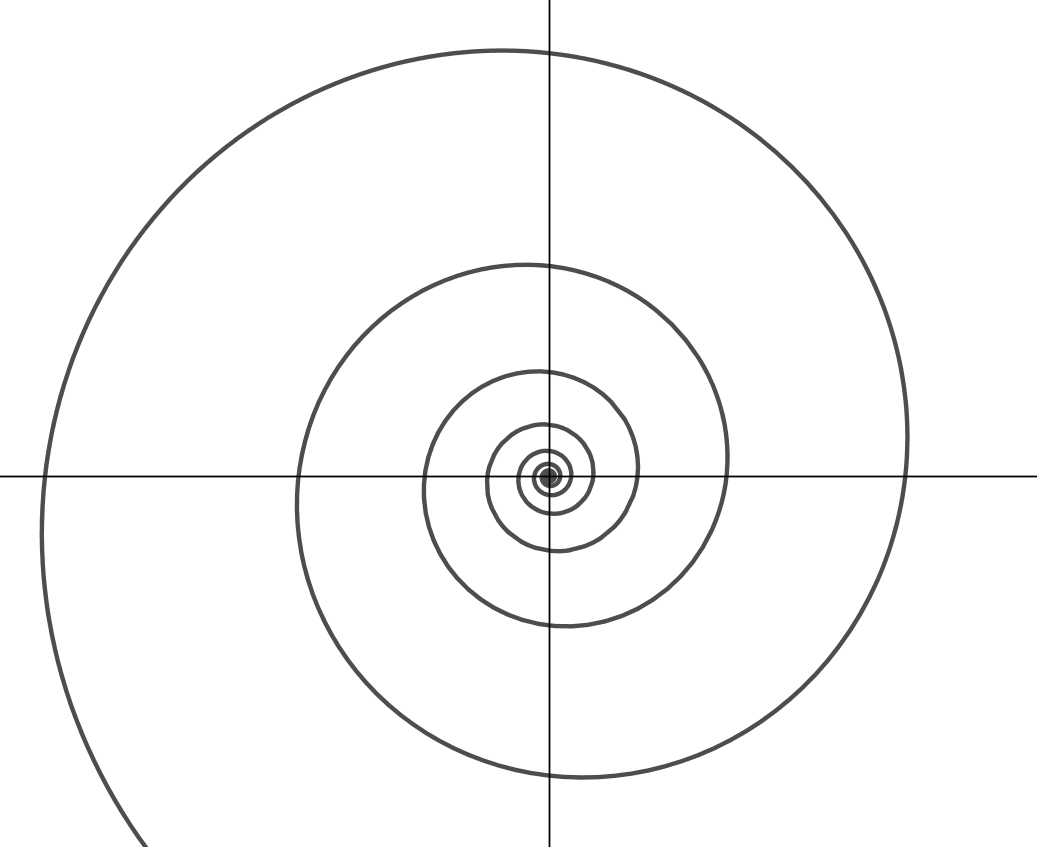
\includegraphics[scale=0.3]{espiral}
\end{figure}


Sea $p=(1,0,0) =\gamma(0)$. Entonces el campo $\gamma'(0)$ tiene coordenadas $\gamma'(0)(x_1)$ y $\gamma'(0)(x_2)$. Vamos a calcularlas. 
\[
\gamma'(0)(x_1)=\left.\frac{d(x_1\circ\gamma)}{dt}\right|_{t=0}=\left.\frac{d(\cos(t)e^t)}{dt}\right|_{t=0}=(-\sin(t)e^t+\cos(t)e^t)_{t=0}=1
\]
\[
\gamma'(0)(x_2)=\left.\frac{d(x_2\circ\gamma)}{dt}\right|_{t=0}=\left.\frac{d(\sin(t)e^t)}{dt}\right|_{t=0}=(\cos(t)e^t+\sin(t)e^t)_{t=0}=1
\]
Luego tenemos el vector tangente $u=\left(\parcial{}{x_1}\right)_p+\left(\parcial{}{x_2}\right)_p$. Este resultado también tiene una interpretación geométrica. Sabemos que el espacio tangente a $S^1\times\R$ en $p$ es isomorfo a $\R\oplus\R$, luego el vector tangente en $p$ tiene la misma componente en cada sumando, lo cual en este caso coincide con la dirección del vector visto sobre el cilindro en $\R^3$ si pensamos en $S^1$ y $\R$ como la circunferencia y la generatriz que pasan por $p$, que sería el $(0,1,1)$. 

\item  La curva $\beta(t)=(1, 0, t)$ para $t\in\R$ es una curva diferenciable sobre el cilindro. Sea $p=(1,0,1)=\beta(1)$. Calculamos las coordenadas del vector $\beta'(1)$.
\[
\beta'(0)(x_1)=\left.\frac{d(1\cdot e^t)}{dt}\right|_{t=1}=e
\]
\[
\beta'(0)(x_2)=\left.\frac{d(0\cdot e^t)}{dt}\right|_{t=0}=0
\]
Entonces el vector es $\beta'(1)=e\left(\parcial{}{x_1}\right)_p$. 

\item La curva $\sigma(t)=(\cos t, \sin t, t^2)$, $t\in\R$, es una curva diferenciable sobre el cilindro. Sea $p=(-1,0,\pi^2)=\sigma(\pi)$. Las coordenadas del vector $\sigma'(\pi)$ son
\[
\sigma'(0)(x_1)=\left.\frac{d(\cos(t) e^{t^2})}{dt}\right|_{t=\pi}=(-\sin(t)e^{t^2}+2t\cos(t)e^{t^2})|_{t=\pi}=-2\pi e^{\pi^2}
\]
\[
\sigma'(0)(x_2)=\left.\frac{d(\sin(t) e^{t^2})}{dt}\right|_{t=\pi}=(\cos(t)e^{t^2}+2t\sin(t)e^{t^2})|_{t=\pi}=-e^{\pi^2}
\]

\end{enumerate}


\section{El cilindro es subvariedad regular de $\R^3$ con la inclusión}


Sea $i:C\hookrightarrow \R^3$ la inclusión. Tal como hemos definido $C$, tiene la topología relativa de $\R^3$, por lo que en virtud de la proposición 4.2.2 de la asignatura Variedades Diferenciables, es suficiente probar que $(C,i)$ es subvariedad de $\R^3$. Para ello probaremos que $i$ es una inmersión inyectiva. Que es inyectiva es evidente, y para que sea inmersión necesitamos que su diferencial lo sea, así que calculamos la matriz de la aplicación $i_{*p}$ para un punto $p\in C$ genérico, que coincide con la matriz jacobiana de la aplicación $i\circ \varphi^{-1}_i$, donde $\varphi_i$ proviniene de la carta que contiene a $p$. Suponemos $i=1$ y el resto de casos son análogos. Por tanto, obtenemos la matriz
\[
\begin{pmatrix}
-\sin\theta & 0 \\
\cos\theta & 0\\
0 & 1
\end{pmatrix}
\]
Esta matriz representa una aplicación lineal $\R^2\to\R^3$ y tiene rango máximo, por lo que efectivamente es inyectiva, con lo que tenemos el resultado. 

\section{Campos diferenciables sobre el cilindro}

Damos tres ejemplos de campos de vectores diferenciables sobre el cilindro. Para los dos primeros usaremos la estrategia de cubrir el cilindro por una familia de curvas diferenciables disjuntas, de modo que en cada punto podemos asociar el vector tangente a ese punto obtenido a partir de la curva que pasa por él. Para el tercero induciremos en $C$ un campo de vectores a partir del campo de vectores de posición de $\R^2\setminus\{0\}$ mediante $\psi$. Igual que para los vectores tangentes, usamos el sistema de coordenadas $(C,\psi=(x_1,x_2))$. 

\begin{enumerate}
\item
 Recordemos la curva $\beta(t)=(1,0,t)$, que es una recta vertical con $t\in\R$. Podemos cubrir el cilindro si hacemos girar esta recta mediante un parámetro $\theta\in[0,2\pi)$, de modo que obtenemos la familia $\beta_\theta(t)=(\cos\theta,\sin\theta, t)$. Para cada punto $p\in C$, existe un único par  $(\theta_0,t_0)$ tal que $p=\beta_{\theta_0}(t_0)$, por lo que definimos el campo $X:C\to TC$ como $X_p=\beta'_{\theta_0}(t_0)$.
 
\item Hacemos ahora lo propio con la familia de circunferencias $\gamma_h(t)=(\cos t,\sin t, h)$ para $t\in (0,2\pi)$ y $h$ variando en $\R$. La diferencia ahora es que esta familia no cubre por completo el cilindro, pero podemos definir el campo de vectores sobre la recta que queda sin cubrir simplemente tomando límite. Es decir, como tenemos que $\lim_{t\to 0^+}\gamma'_h(t)=\lim_{t\to 2\pi^-}\gamma'_h(t)=-e^h\left(\parcial{}{x_2}\right)_p$, donde $p=(1,0,h)$, tenemos un vector tangente para cada punto de dicha recta, al que denotaremos $\gamma'_h(0)$. Así, definimos el campo $Y:C\to TC$ como $Y_p=\gamma'_{h_0}(t_0)$, donde $(h_0, t_0)$ es el único par tal que o bien $\gamma_{h_0}(t_0)=p$ o bien $t=0$ y $p=(1,0,h_0)$. 

\item Sea $\R^2\setminus\{0\}$ con coordenadas $(u_1,u_2)$ dadas por la identidad. Consideramos el campo $X_p=u_1(p)\left(\parcial{}{u_1}\right)_p+u_2(p)\left(\parcial{}{u_2}\right)_p$. Transformamos este campo sobre $\R^2\setminus\{0\}$ en un campo sobre $C$ mediante el $\psi^{-1}_*:\mathcal{X}(C)\to\mathcal{X}(\R^2\setminus\{0\})$. Recordamos que en el cilindro tenemos coordenadas $(x_1,x_2)$. Por definición, 
\[
(\psi^{-1}_*X)x_i=X(x_i\circ \psi^{-1})\circ \psi=X(u_i)\circ\psi =u_i\circ\psi 
\]
que para $i=1$ nos da $xe^z$ y para $i=2$, $ye^z$. Es decir, para un punto $p=(x,y,z)\in C$, $(\psi^{-1}_*X)_p$ tiene la expresión local
\[
xe^z\left(\parcial{}{x_1}\right)_p+ye^z\left(\parcial{}{x_2}\right)_p.
\]
\end{enumerate}

\section{Métrica Riemanniana sobre el cilindro}

Como hemos visto anteriormente, $(C,i)$ es una subvariedad regular de $\R^3$. En particular, $i:C\to \R^3$ es una inmersión, luego el pull-back $i^*g$, donde $g$ es la métrica usual de $\R^3$, define una métrica riemanniana sobre $C$ tal como se ha visto en clase.


\section{Ejemplos de geodésicas}




\section{Curvatura escalar del cilindro}

\end{document}
